\documentclass[12pt,a4paper]{article}
\usepackage{amsmath}
\usepackage{amsthm}
\usepackage{amsfonts}
\usepackage{amssymb}
\usepackage{amsmath,amscd}
\usepackage{fancyhdr}
\usepackage{graphicx}
\usepackage{bm}
\usepackage{caption}
\usepackage{floatpag}
\usepackage[english]{babel}
\linespread{1}

\newtheorem{theo}{Theorem}
\newtheorem{lem}{Lemma}
\newtheorem{prop}{Proposition}
\newtheorem{cor}[theo]{Corollary}
\newtheorem{defn}{Definition}
\newtheorem{con}{Conjecture}

\DeclareMathOperator{\Tr}{Tr}
\DeclareMathOperator{\Real}{Re}
\newcommand{\eit}{e^{i \theta}}
\newcommand{\eits}{e^{2i \theta}}
\newcommand{\emit}{e^{-i \theta}}
\newcommand{\emits}{e^{-2i \theta}}

\renewcommand{\thefootnote}{\fnsymbol{footnote}}

% Title
\title{$1^{st}$ year PhD report}
\author{Mauro D'Arcangelo \\ Supervisor: Prof. J. W. Barrett}
\date{}

\begin{document}

\maketitle


% Table of contents
\tableofcontents
\newpage

% Sections
\section{Introduction}\label{intro}
This project is concerned with the characterization of \emph{random fuzzy spaces} by means of Markov chain Monte Carlo simulations. The chapter presents a brief introduction to the basic concepts (non-commutative, fuzzy and random).

\subsection{Non-commutative geometry} \label{sec:ncg}
The fundamental object of non-commutative geometry is a \emph{spectral triple} $(A, H, D)$ where $A$ is an algebra with a representation in a Hilbert space $H$ and $D$ is an operator on $H$, called Dirac operator. A Riemannian spin manifold can be fully characterized by the commutative algebra $A$ of functions on the manifold and by the Dirac operator, which encodes the metric \cite{connesRECON}. One could then consider a generalization in which the algebra is allowed to be non-commutative. Such geometries arise naturally in physics, and are tightly related to gauge theories \cite{suijlekom}. Indeed it has been shown that the Standard Model has the structure of a non-commutative geometry \cite{barrettLOR} \cite{connesSAP} \cite{connesNEUT} \cite{connesGRAVMAT}. This suggests a possible path to quantum gravity by replacing the ordinary commutative spacetime by a non-commutative one that presents a commutative behaviour as a limiting case.

\subsection{Fuzzy spaces} \label{sec:fuzzy}
There is a class of non-commutative geometries called \emph{fuzzy spaces}, where the algebra is taken to be $M_n(\mathbb{C})$, the algebra of $n \times n$ complex matrices, and the Hilbert space is finite dimensional. The Dirac operator of a fuzzy space takes the form \cite{barrett}:
\begin{equation}\label{eq:dirac_bad}
D = \sum_j \alpha_j \otimes [L_j, \cdot ] + \sum_k \tau_k \otimes \{H_k, \cdot \}
\end{equation}
where:
\begin{enumerate}
\item  $\tau_k$ and $\alpha_j$ are respectively Hermitian and anti-Hermitian basis elements of the algebra generated by a $(p, q)$ Clifford module;
\item $H_k$ and $L_j$ are $n \times n$ Hermitian and anti-Hermitian matrices respectively;
\item $[\cdot , \cdot]$ indicates a commutator and $\{ \cdot , \cdot \}$ an anti-commutator.  
\end{enumerate}
Fuzzy spaces are classified by the pair of integers $(p, q)$ of the Clifford module. It is worth noting that any choice of $H_k$ and $L_j$ gives an admissible Dirac operator, as long as the Hermitian or anti-Hermitian character is preserved.\newline
See Appendix A for some remarks on the notation used.

\subsection{Random geometries} \label{sec:rand}
A \emph{random geometry} is a spectral triple $(A, H, D)$ in which the Dirac operator fluctuates according to a certain probability measure. Here the probability measure is taken to be proportional to:
\begin{equation} \label{eq:prob}
e^{-S[D]} d D
\end{equation}
for a certain choice of $S[D]$. The expectation value of an observable $f(D)$ on a random geometry is given by:
\begin{equation} \label{eq:expval}
\langle f(D) \rangle = \int f(D) e^{-S[D]} d D.
\end{equation}
Since $D$ encodes the metric, this is in clear analogy with the Euclidean path integral of Quantum Field Theory. \newline
So far no assumption has been made on the choice of Dirac operator. The purpose of this project is to study the path integral when $D$ is taken to be the Dirac operator of a fuzzy space.\newline
Fuzzy spaces provide an alternative type of regularization that is non-lattice \cite{barrettglaser}. Therefore the study of such random geometries is especially interesting in connection with models of (Euclidean) quantum gravity. \newline
This line of research first appeared in \cite{barrettglaser}, where the following action was considered:
\begin{equation}\label{eq:action}
S[D] = g_2 \Tr D^2 + \Tr D^4, \quad g_2 \in \mathbb{R}.
\end{equation}
In the remainder, the action is taken to be of the form of Eq.(\ref{eq:action}).\newline
The expectation value (\ref{eq:expval}) is computed numerically using Monte Carlo methods. Eq.(\ref{eq:expval}) is therefore replaced by:
\begin{equation} \label{eq:expval_mc}
\langle f(D) \rangle \approx  \frac{1}{N}\sum_{i=1}^N f(D_i)
\end{equation}
where $\{D_i\}$ is a set of Dirac operators sampled from the distribution (\ref{eq:prob}).



\newpage

\section{Results}\label{results}
\subsection{Improvements in the numerical algorithm}
The evaluation of integrals such as (\ref{eq:expval}) requires a way to sample the most relevant configurations (the \textit{typical set}) out of the entirety of parameter space. The simplest algorithm based on Markov chains for doing so is Metropolis-Hastings \cite{hastings}. Two crucial shortcomings of Metropolis are a rather slow exploration of the typical set based on a random walk in parameter space, and the large correlation between adjacent samples. A more sophisticated approach is Hybrid Monte Carlo, or HMC \cite{duane}: originally developed for lattice QCD computations, it allows a faster and more uniform exploration of the typical set by transposing the problem of sampling from a distribution to Hamiltonian evolution in a fictitious phase space.\newline
After a brief explanation of the idea behind HMC, the adaptation to the fuzzy space path integral is discussed and the results from numerical simulations are presented with a comparison between HMC and Metropolis.

\subsubsection{Hybrid Monte Carlo}
In Markov chain theory one is interested in a system specified by a finite set of parameters $(q_1, \cdots, q_N), \ q_i \in \mathbb{R}$, collectively referred to as $\mathbf{q}$. The probability that the system be in a particular configuration is given by some probability measure $\pi (\mathbf{q}) d\mathbf{q}$. Given an initial configuration $\mathbf{q}$, a Markov chain establishes a transition $\mathbf{q} \rightarrow \mathbf{q}'$ from the old configuration to a new one in such a way that $\mathbf{q}'$ is chosen with the desired probability.\newline 
This situation is analogous to the Monte Carlo estimation of the integral (\ref{eq:expval}), where the parameters are the independent degrees of freedom of the Dirac operator and the probability measure is $e^{-S[D]}dD$.\newline
The first step of Hybrid Monte Carlo is to enlarge parameter space by introducing a ``conjugate momentum'' $p_i$ to each parameter $q_i$, thus effectively working in a fictitious phase space. The probability measure is extended to include the new variables $\pi (\mathbf{q}) \rightarrow \pi (\mathbf{q}, \mathbf{p})$. By defining the ``Hamiltonian'' $H(\mathbf{q}, \mathbf{p}) \equiv -\log \pi (\mathbf{q}, \mathbf{p})$, a configuration is then evolved along a Hamiltonian trajectory by integrating Hamilton's equations:
\begin{align}
\frac{dq_i}{dt} &= \frac{\partial{H}}{\partial{p_i}} \label{eq:dqdt} \\
\frac{dp_i}{dt} &= -\frac{\partial{H}}{\partial{q_i}} \label{eq:dpdt}
\end{align}
where $t$ denotes a fictitious time that will be referred to as Monte Carlo time. This specifies a transition $(\mathbf{q}(0), \mathbf{p}(0)) \rightarrow (\mathbf{q}(t), \mathbf{p}(t))$ from an initial configuration to a new one. The new configuration is then accepted with probability $\text{min}[1, \exp (H(t)-H(0))]$. \newline
Note that Hamiltonian dynamics preserves the value of the energy of the system, therefore $H(t) = H(0)$ and $\text{min}[1, \exp (H(t)-H(0))] = 1$. However, numerical integration of Hamilton's equations is a non-trivial matter that introduces errors, therefore $H(t) \neq H(0)$ in general. The standard choice of numerical integrator in HMC is the so-called \textit{leapfrog} integrator \cite{neal} \cite{betan}.

\subsubsection{Adapting HMC to fuzzy spaces}
In the matrix integral considered here, the dynamical variables are the $n \times n$ Hermitian matrices $M_i$, to which a corresponding set of Hermitian matrices $P_i$ is added. The Hamiltonian is chosen to be simply:
\begin{equation} \label{eq:hamilt}
H(M_i, P_i) = S[M_i] + \sum_i \frac{1}{2}P_i^2.
\end{equation}
Schematically, the algorithm goes as follows:
\begin{enumerate}
\item extract the momenta $P_i$ according to $\exp(-P_i^2 / 2)$;
\item integrate Hamilton's equations for a certain time $t$;
\item accept the new configuration with probability $\text{min}[1, \exp (H(t)-H(0))]$.
\end{enumerate}
The non-trivial step in the leapfrog integrator is the evaluation of the force term in Eq.(YYYY), which requires to take derivatives such as:
\begin{equation}
\frac{\partial S[M_i]}{\partial M_k}
\end{equation}
which amounts to finding formulas for terms like:
\begin{equation}
\frac{\partial \Tr D(M_i)^p}{\partial M_k}.
\end{equation}
For the definition of matrix derivative see Appendix B. In the following, formulas for $p=2$ and $p=4$ are developed.

\subsubsection{The case $p=2$}
When $p = 2$ the $M_i$ matrices are decoupled:
\begin{equation}
\Tr D^2 = \sum_i \Tr \omega_i^2 (2 n \Tr M_i^2 + 2 \epsilon_i (\Tr M_i)^2).
\end{equation} 
Taking a derivative with respect to $M_k$ yields:
\begin{align}\label{eq:As}
\frac{\partial}{\partial M_k} \left( \sum_i \Tr \omega_i^2 (2 n \Tr M_i^2 + 2 \epsilon_i (\Tr M_i)^2) \right) = \notag \\
\sum_i \delta_{ik} \Tr \omega_i^2 \left( 4 n M_i^T + 4 \epsilon_i (\Tr M_i) I \right) = \notag \\
4 C \left( n M_k^T + \epsilon_k (\Tr M_k) I \right)
\end{align}
where $C \equiv \Tr \omega_i^2$ is the dimension of the Clifford module.

\subsubsection{The case $p=4$}
First expand $\Tr D^4$:
\begin{align}\label{eq:trd4}
\Tr D^4 &= \sum_{i_1, i_2, i_3, i_4} \Tr (\omega_{i_1} \omega_{i_2} \omega_{i_3} \omega_{i_4}) \cdot \notag \\
\Big( \ &n [1+\epsilon \ *] \Tr (M_{i_1} M_{i_2} M_{i_3} M_{i_4})  \ \  + \notag \\
&\epsilon_{i_1} \Tr M_{i_1} [1 + \epsilon \ *] \Tr ( M_{i_2} M_{i_3} M_{i_4})  \ \  + \notag \\
&\epsilon_{i_2} \Tr M_{i_2} [1  + \epsilon \ *] \Tr (M_{i_1} M_{i_3} M_{i_4}) \ \  + \notag \\
&\epsilon_{i_3} \Tr M_{i_3} [1 + \epsilon \ *] \Tr (M_{i_1} M_{i_2} M_{i_4})  \ \  + \notag \\
&\epsilon_{i_4} \Tr M_{i_4} [1 + \epsilon \ *] \Tr (M_{i_1} M_{i_2} M_{i_3})  \ \  + \notag \\
&\epsilon_{i_1} \epsilon_{i_2} [1 + \epsilon] \Tr (M_{i_1} M_{i_2} ) \Tr (M_{i_3} M_{i_4})   \ \  + \notag \\
&\epsilon_{i_1} \epsilon_{i_3} [1 + \epsilon] \Tr (M_{i_1} M_{i_3}) \Tr (M_{i_2} M_{i_4})   \ \  + \notag \\
&\epsilon_{i_1} \epsilon_{i_4} [1 + \epsilon] \Tr (M_{i_1} M_{i_4}) \Tr (M_{i_2} M_{i_3})   \ \Big)
\end{align}
where $*$ denotes complex conjugation of everything that appears on the right, $\epsilon$ is defined as the product $\epsilon \equiv \epsilon_{i_1}\epsilon_{i_2}\epsilon_{i_3}\epsilon_{i_4}$, and the relation $M^T = M^*$ has been used. Since $D$ is Hermitian, the expression must be real. It is not immediate to see that this is the case because of the $\epsilon = \pm 1$ factor inside the square brackets. Reality nonetheless holds, and becomes manifest by observing that a simultaneous index exchange $i_1 \leftrightarrow i_4$ and $i_2 \leftrightarrow i_3$ is equivalent to taking the complex conjugate (in fact, this is not the only index exchange that amounts to complex conjugation). \newline
Taking a matrix derivative with respect to $M_k$ results in non-vanishing contributions when $k=i_1, k=i_2, k=i_3$ or $k=i_4$:
\begin{align}
\frac{\partial}{\partial M_k} \Tr D^4 &= \sum_{i_1, i_2, i_3, i_4} \Tr (\omega_{i_1} \omega_{i_2} \omega_{i_3} \omega_{i_4}) \cdot \notag \\
\Big( &\delta_{ki_1} A(i_1, i_2, i_3, i_4)^T + \delta_{ki_2} A(i_2, i_3, i_4, i_1)^T + \notag \\
&\delta_{ki_3} A(i_3, i_4, i_1, i_2)^T + \delta_{ki_4} A(i_4, i_1, i_2, i_3)^T \Big)
\end{align}
where $A(a, b, c, d )$ is the following $n \times n$ matrix:
\begin{align}
A(a,b,c,d) \equiv \ &n [1+\epsilon \ \dagger] M_b M_c M_d + \notag \\
&\epsilon_a I [1 + \epsilon \ *] \Tr M_b M_c M_d  + \notag \\
&\epsilon_b \Tr M_b [1 + \epsilon \ \dagger] M_c M_d + \notag \\
&\epsilon_c \Tr M_c [1 + \epsilon \ \dagger] M_b M_d + \notag \\
&\epsilon_d \Tr M_d [1 + \epsilon \ \dagger] M_b M_c + \notag \\
&\epsilon_a \epsilon_b M_b [1 + \epsilon] \Tr M_c M_d + \notag \\
&\epsilon_a \epsilon_c M_c [1 + \epsilon] \Tr M_b M_d + \notag \\
&\epsilon_a \epsilon_d M_d [1 + \epsilon] \Tr M_b M_c
\end{align}
and $\dagger$ denotes Hermitian conjugation of everything that appears on the right. Upon relabeling the indices and cycling the $\omega$ matrices in the trace, the equation becomes:
\begin{align}\label{eq:derd4}
\frac{\partial}{\partial M_k} \Tr D^4 &= 4 \sum_{i_1, i_2, i_3, i_4} \delta_{ki_1} \Tr (\omega_{i_1} \omega_{i_2} \omega_{i_3} \omega_{i_4}) A(i_1, i_2, i_3, i_4)^T \notag \\
&= 4 \sum_{i_1, i_2, i_3} \Tr (\omega_{k} \omega_{i_1} \omega_{i_2} \omega_{i_3}) A(k, i_1, i_2, i_3)^T \equiv 4 \sum_{i_1, i_2, i_3} \mathcal{B}_k(i_1, i_2, i_3)
\end{align}
with $\mathcal{B}_k(a, b, c)$ denoting the generic term in the sum.\newline
To see that Eq.(\ref{eq:derd4}) defines a Hermitian matrix, notice that an exchange of indices $i_1 \leftrightarrow i_3$ is equivalent to taking the Hermitian conjugate:
\begin{equation}\label{eq:BBd}
\mathcal{B}_k(i_1, i_2, i_3)^{\dagger} = \mathcal{B}_k(i_3, i_2, i_1)
\end{equation}
therefore the sum in Eq.(\ref{eq:derd4}) reduces to:
\begin{equation}\label{eq:splitsum}
\sum_{\substack{i_1 > i_3 \\ i_2}} [1+\dagger] \mathcal{B}_k(i_1, i_2, i_3) + \sum_{i_1, i_2} \mathcal{B}_k(i_1, i_2, i_1).
\end{equation}
In fact, by looking at the form of $\mathcal{B}$, it is clear that terms in the sum are qualitatively different based on the number of indices that coincide. Therefore it would be computationally convenient to write Eq.(\ref{eq:splitsum}) in a way that emphazises this difference.\newline
The only terms that contribute when all indices are different are the following:
\begin{equation} \label{eq:alldifferent}
\sum_{i_1 > i_2 > i_3} [1+\dagger] \Big( \mathcal{B}_k(i_1, i_2, i_3) + \mathcal{B}_k(i_1, i_3, i_2) + \mathcal{B}_k(i_2, i_1, i_3) \Big).
\end{equation}
The three inequivalent permutations of indices that appear in this formula are based on a group-theoretical argument that will generalize easily to powers of $D$ higher than 4. First consider the symmetric group of order three $S_3$ acting on the set of indices $\{i_1, i_2, i_3\}$, and the subgroup of permutations that induce a simple change in $\mathcal{B}$, which in this case is $H = \{(), (13)\} \cong S_2$ (the first element being the identical permutation, and the second the exchange $i_1 \leftrightarrow i_3$ which induces $\mathcal{B} \rightarrow \mathcal{B}^\dagger$). The idea is then to restrict the sum to $i_1 > i_2 > i_3$ and quotient out the action of $H$ by introducing a suitable pre-factor that accounts for it (in this case $[1+\dagger]$). Practically, the inequivalent permutations of indices that appear in Eq.(\ref{eq:alldifferent}) are found by computing the (left or right) cosets of $H \subset S_3$ and acting on $\{i_1, i_2, i_3\}$ with a representative from each coset. In this case the representatives where chosen to be $(), (23), (12)$.\newline
What is left are terms in which at least two indices are equal. These are:
\begin{align} \label{eq:someequal}
\sum_{i_1 > i_2} [1+\dagger] \Big( \mathcal{B}_k(i_1, i_1, i_2) &+ \mathcal{B}_k(i_1, i_2, i_2) \Big) + \notag \\
&\sum_{i_1 \neq i_2} \mathcal{B}_k(i_1, i_2, i_1) + \sum_{i} \mathcal{B}_k(i,i,i).
\end{align}
At this point, a useful property of the $\omega$ matrices can be exploited to simplify both Eq.(\ref{eq:alldifferent}) and Eq.(\ref{eq:someequal}):
\begin{equation}\label{eq:gamma0}
\Tr(\omega_{\sigma(i_1)} \omega_{\sigma(i_2)} \omega_{\sigma(j)} \omega_{\sigma(k)}) \propto \Tr(\omega_j \omega_k) = 0 \qquad \text{if} \ \ i_1 = i_2 \ \text{and} \ j \neq k
\end{equation}
for any permutation $\sigma$ acting on $\{i_1, i_2, j, k\}$. In other words, if two indices are the same and the other two are different, the trace on the $\omega$ matrices vanishes.\newline
Putting together Eq.(\ref{eq:alldifferent}), Eq.(\ref{eq:someequal}) and Eq.(\ref{eq:gamma0}), the final formula for $\partial_k \Tr D^4$ reads:
\begin{align} 
\frac{\partial}{\partial M_k} \Tr D^4 = 4 \Bigg[ \sum_{\substack{i_1 > i_2 > i_3 \\ i_1,i_2,i_3 \neq k}} &[1+\dagger] \Big( \mathcal{B}_k(i_1, i_2, i_3) + \mathcal{B}_k(i_1, i_3, i_2) + \mathcal{B}_k(i_2, i_1, i_3) \Big) \notag \\
&+ \sum_{\substack{i \\ i \neq k}} \Big( [1+\dagger] \mathcal{B}_k(i, i, k) + \mathcal{B}_k(i, k, i) \Big) + \mathcal{B}_k(k,k,k) \Bigg].
\end{align}
The explicit form of $\mathcal{B}_k(i,i,k), \ \mathcal{B}_k(i,k,i)$ and $\mathcal{B}_k(k,k,k)$ is given in Appendix C.

\subsubsection{Testing HMC against exact results}
Although not many analytical results are available for the matrix integrals considered here, there is a non-trivial observable whose expectation value is known exactly for any geometry and any action polinomial in $D$. Computing this observable therefore provides a good test for the numerical implementation.\newline
Consider the following vanishing integral:
\begin{equation} \label{eq:vanint}
0 = \int \frac{\partial}{\partial D_{ij}} \left( D_{ij} e^{-S[D]} \right) d D
\end{equation}
where $D_{ij}$ is one of the independent degrees of freedom of the Dirac operator and $S[D]$ is in general sum of terms like $g_p \Tr D^p$.\newline
An explicit calculation of the right-hand side of Eq.(\ref{eq:vanint}) gives:
\begin{equation}
0 = \int \left( 1 - \sum_p g_p D_{ij} \frac{\partial}{\partial D_{ij}} \Tr D^p \right) e^{-S[D]}d D
\end{equation}
dividing by the partition function and rearranging the terms:
\begin{equation}
1 =\frac{1}{\int e^{-S[D]}} \int \left( \sum_p g_p D_{ij} \frac{\partial}{\partial D_{ij}} \Tr D^p \right) e^{-S[D]}d D
\end{equation}
and finally summing over all $i, j$ corresponding to independent degrees of freedom:
\begin{equation}\label{eq:dofs}
\#\text{d.o.f.}(D) = \frac{1}{\int e^{-S[D]}} \int \left( \sum_p g_p \ p \Tr D^p \right) e^{-S[D]} d D = \left\langle \sum_p g_p \ p \  \Tr D^p \right\rangle
\end{equation}
where the following identity, a proof of which is given in Appendix D, was used:
\begin{equation}
\sum_{ij} D_{ij} \frac{\partial}{\partial D_{ij}} \Tr D^p = p \Tr D^p.
\end{equation}
To estimate the number of degrees of freedom recall that in the decomposition (\ref{eq:dirac}) the $M_i$ matrices are all Hermitian, therefore {\#}d.o.f.$(D) = n^2m$ where $n$ is the dimension and $m$ the total number of $M_i$ matrices.\newline
Numerical tests of HMC and Metropolis agree with the prediction (\ref{eq:dofs}). As an example, a test on the $(0,3)$ Dirac operator is reported in Fig.(\ref{fig:dofs}).
\begin{figure}[hp]
\centering
\textbf{$\text{\# dofs} = 2 g_2 \langle S_2 \rangle + 4\langle S_4 \rangle$ test: comparison Metropolis/HMC}
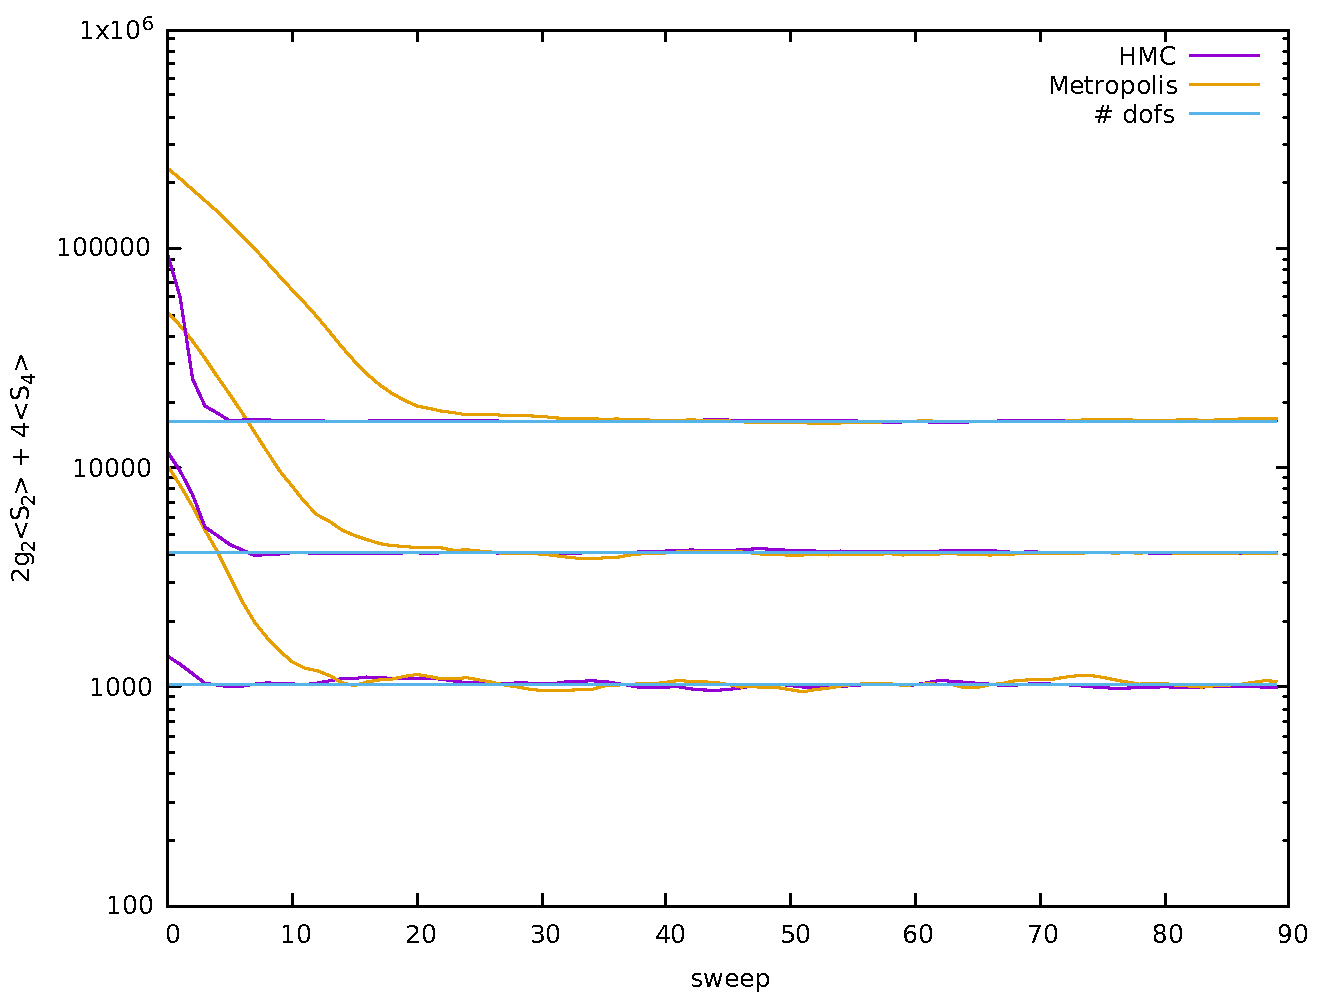
\includegraphics[width=1\linewidth]{fig/dofsp0q3.pdf}
\caption{Convergence of the expectation value of the observable $2 g_2 \Tr D^2 + 4 \Tr D^4 $ to the number of degrees of freedom of the Dirac operator for geometry $(0,3)$. The three sets correspond to matrix size $n = 16 \times 16$, $32 \times 32$ and $64 \times 64$. }
\label{fig:dofs}
\end{figure}

\subsubsection{Comparing the speed of HMC and Metropolis}
The samples produced by a Markov chain are correlated with each other. In general HMC generates less correlated samples if compared to Metropolis, resulting in higher quality data for a given computational cost.\newline
When computing a specific observable $O$, the efficiency of an algorithm in producing uncorrelated samples can be quantified by the \textit{time-displaced autocorrelation}:
\begin{equation}
\chi(t) = \int dt' O(t')O(t'+t) - \langle O \rangle^2
\end{equation}
where $O(t)$ represents the value of the observable at Monte Carlo time $t$. The autocorrelation function is expected to fall off exponentially:
\begin{equation}
\chi(t) \sim e^{-\frac{t}{\tau}}
\end{equation}
and $\tau$ is known as the autocorrelation time. Two values of the observable taken at $\sim 2\tau$ distance from each other are considered independent.\newline
The autocorrelation time tends to be dramatically larger near second-order phase transitions. For this reason the $(2,0)$ geometry at the phase transition was chosen to test HMC against Metropolis. The order parameter for the phase transition is:
\begin{equation}
F = \frac{(\Tr H_1)^2 + (\Tr H_2)^2}{n( \Tr H_1^2 + \Tr H_2^2)}
\end{equation}
where $H_i$ are the two free Hermitian matrices of the model. The plot of the time-displaced autocorrelation and the exponential fit for HMC and Metropolis are reported in Fig.(\ref{fig:autoc}). The exponential fit gives an autocorrelation time of $\sim 250$ sweeps for Metropolis and $\sim 25$ sweeps for HMC, meaning that in this example Metropolis needs to run 10 times longer than HMC for collecting the same amount of independent samples.
\begin{figure}[hp]
\centering
\textbf{Autocorrelation of order parameter $(2,0)$ test: comparison Metropolis/HMC}
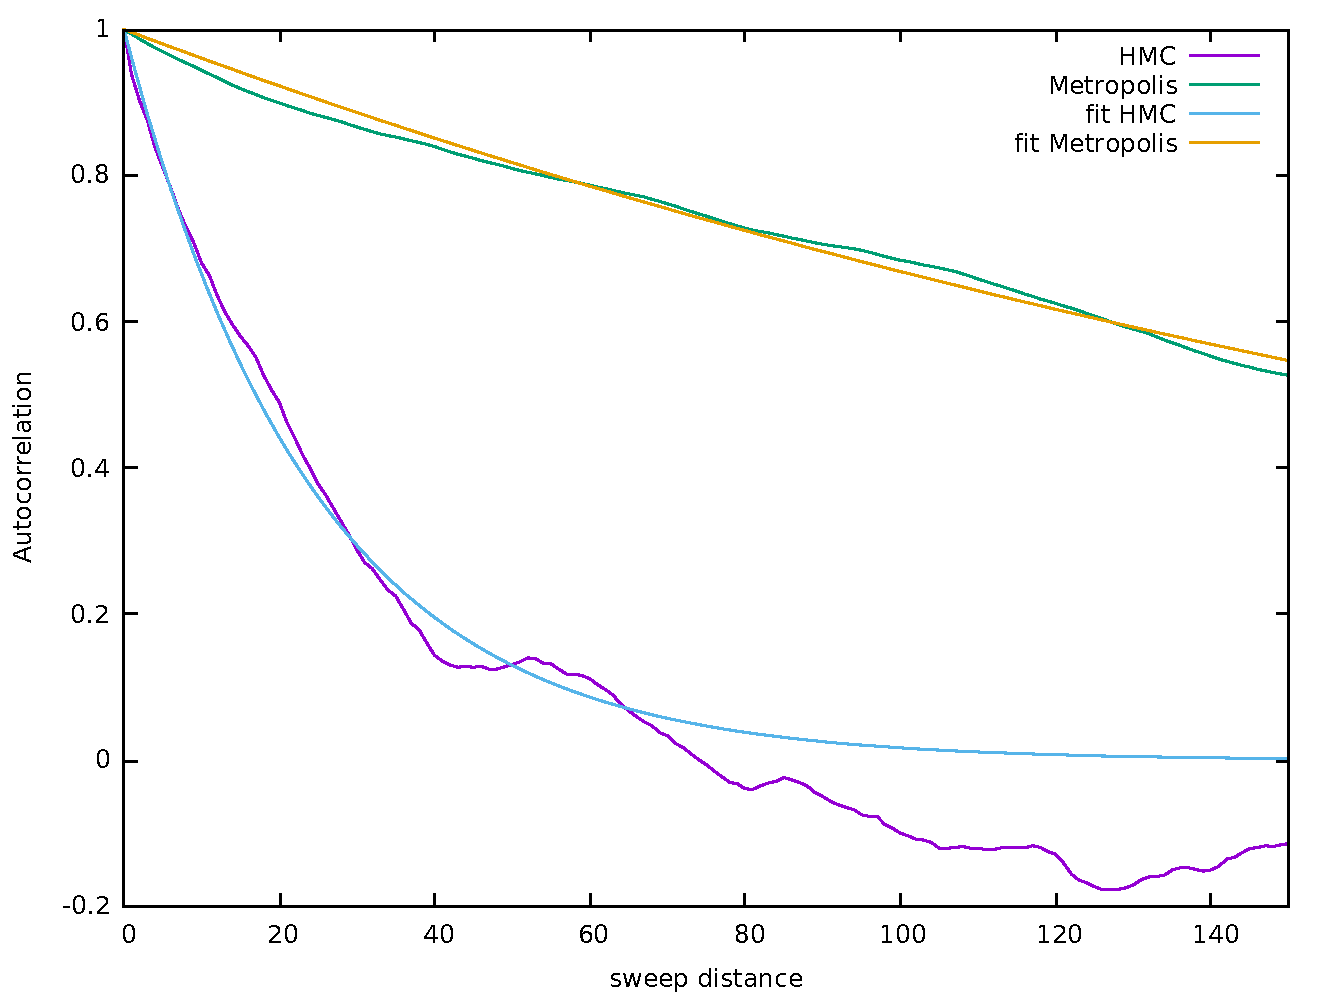
\includegraphics[width=1\linewidth]{fig/autocorrp2q0.pdf}
\caption{Autocorrelation $\chi (t)$ (normalized by $\chi(0)$) of the $(2,0)$ phase transition order parameter $F$. The coupling constant $g_2 = 2.725$ was chosen to be at the phase transition. The exponential fit gives an autocorrelation time of $\sim 250$ sweeps for Metropolis and $\sim 25$ sweeps for HMC.}
\label{fig:autoc}
\end{figure}
\newline
Of course Metropolis might be more than 10 times faster than HMC to collect a single sample, therefore the raw speed of the algorithm needs to be taken into account as well. In order to test this, the speed of HMC and Metropolis in generating 100 samples for the $(0,3)$ geometry was recorder for matrix dimension $16 \times 16$, $32 \times 32$ and $64 \times 64$. The results are reported in Tab.(\ref{tab:speed}).\newline
For small matrix size the two algorithms are comparable in speed, while for larger matrices HMC greatly outperforms Metropolis. Linearly fitting the data in logaritmic scale allows to estimate how the two algorithms scale with the matrix dimension, giving a computational cost of $O(n^{4.6})$ and $O(n^{2.6})$ for Metropolis and HMC respectively.
\begin{table}[hp]
\centering
\begin{tabular}{|l|l|l|}
\hline
\begin{tabular}[c]{@{}l@{}}Matrix\\ dimension\end{tabular} & \begin{tabular}[c]{@{}l@{}}time\\ HMC (sec)\end{tabular} & \begin{tabular}[c]{@{}l@{}}time\\ Metropolis (sec)\end{tabular} \\ \hline
16 & 23 & 17 \\ \hline
32 & 100 & 428 \\ \hline
64 & 1612 & 21218 \\ \hline
\end{tabular}
\caption{Time for 100 sweeps of HMC and Metropolis for geometry $(0,3)$. Fitting of the data gives a computational cost of $O(n^{4.6})$ and $O(n^{2.6})$ for Metropolis and HMC respectively.}
\label{tab:speed}
\end{table}



\newpage
\subsection{Yang-Mills matrix models from Dirac operators}
Yang-Mills matrix models have been studied extensively in the past \cite{ymnum1} \cite{ymnum2} \cite{ymnum3} \cite{ymnum4} as models of emergent geometry. Fuzzy spaces arise as classical solutions, and perturbations around them give rise to non-commutative gauge theories \cite{hareview}.\newline
The purpose of this section is to show a formal similarity between Yang-Mills matrix models and a certain choice of Dirac operator, despite the very different origin of the two models.\newline

\subsubsection{Yang-Mills matrix models}
A Yang-Mills matrix model is given by the following action:
\begin{equation}\label{eq:ymaction}
S \propto -\frac{1}{4} \Tr [M_i, M_j]^2 + \frac{2}{3} i g_3 \epsilon_{ijk} \Tr M_i M_j M_k + \frac{1}{2} g_2 \Tr M_i^2
\end{equation}
where $M_i, i=1,2,3$, are $n \times n$ Hermitian matrices and a sum is intended on repeated indices. Actions without the quadratic or cubic term can also be considered. Note that in general one can consider models with more than three matrices (for example the IKKT model \cite{ikkt} has 10 matrices).\newline
The variation of this action gives the following classical equation of motion for the generic matrix $M_i$:
\begin{equation}\label{eq:ymeom}
[M_j, [M_j, M_i]] + i g_3 \epsilon_{ijk}[M_j, M_k] + g_2 M_i = 0
\end{equation}
where again sum on repeated indices is implied. Diagonal matrices satisfy Eq.(\ref{eq:ymeom}), but a more interesting class of solutions is given by matrices forming an $n$-dimensional representation of the $su(2)$ Lie algebra:
\begin{equation}\label{eq:ymsol}
[M_i, M_j] = i \epsilon_{ijk} M_k.
\end{equation}
In this sense fuzzy spheres are classical solutions of (\ref{eq:ymaction}).

\subsubsection{Type $(0,3)$ geometry as a Yang-Mills matrix model}
Consider the following Dirac operator:
\begin{equation}\label{eq:ymdirac}
D = \sum_i \sigma_i \otimes M_i
\end{equation}
where $\sigma_i, \ i=1,2,3$ are the Pauli matrices and $M_i$ are Hermitian matrices. Note that no commutators or anti-commutators appear in the Dirac operator, meaning that the bimodule structure of the algebra on itself is ignored and only the left (or right) action is taken into account. Eq.(\ref{eq:ymdirac}) is nonetheless an example of type $(0,3)$ Dirac operator, although not the most general one.\newline
Consider then the usual action for $D$ (with an additional cubic term and some convenient numerical factors):
\begin{equation}
S[D] = \frac{1}{4} \Tr D^4 + \frac{1}{3}g_3 \Tr D^3 + \frac{1}{4}g_2 \Tr D^2.
\end{equation}
It follows from the properties of the Pauli matrices that such action, rewritten explicitly in terms of the $M_i$ matrices, takes a form very similar to (\ref{eq:ymaction}):
\begin{align}
S[D(M_i)] = &-\frac{1}{4} \Tr [M_i, M_j]^2 -\frac{1}{2} \Tr M_i^2 M_j^2 \\ \notag
&+ \frac{2}{3} i g_3 \epsilon_{ijk} \Tr M_i M_j M_k \\ \notag
&+ \frac{1}{2} g_2 \Tr M_i^2.
\end{align}
The only difference is in fact an extra term $\Tr M_i^2 M_j^2$ in the quartic part. The role of this term becomes clear by writing the equation of motion:
\begin{equation}
[M_j, [M_j, M_i]] - \{M_j^2, M_i \} + i g_3 \epsilon_{ijk}[M_j, M_k] + g_2 M_i = 0
\end{equation}
which still has the $su(2)$ algebra solution (\ref{eq:ymsol}), provided that $\sum_j M_j^2$ is a Casimir. The extra term in the action for the Dirac operator therefore forces the representation to be either irreducible or direct sum of copies of the same irreducible.\newline
It is interesting to see what happens if the commutator structure is reintroduced, so that the Dirac operator is now:
\begin{equation}
D = \sum_i \sigma_i \otimes [M_i,\cdot ]
\end{equation}
which is formally equivalent to replacing $M_i$ with $[M_i, \cdot ]$ in each formula so far. First notice that making this replacement in the equation of motion for $M_i$ and ignoring the extra quartic term $\{[M_j, \cdot ]^2, [M_i, \cdot ] \}$ makes the $su(2)$ algebra still a viable classical solution: 
\begin{equation}
[M_i, M_j] = i \epsilon_{ijk} M_k \ \implies \ [[M_i, \cdot ], [M_j, \cdot ]] = [[M_i, M_j], \cdot ] = i \epsilon_{ijk} [M_k, \cdot ]
\end{equation}
however, the presence the extra quartic term now imposes the much stricter constraint of the representation to be the two-dimensional one (or direct sum of copies thereof). One way to see this is to expand the commutators as in (\ref{eq:acomm}) and calculate the contribution of the extra term explicitly:
\begin{align}\label{eq:exquart}
\{[M_j, \cdot ]^2, [M_i, \cdot ] \} = &\{ \{M_j^2, \cdot\}, [M_i, \cdot ] \} \\ \notag
& -2 \{ M_i , M_j \} \otimes M_j^T + 2 M_j \otimes \{ M_i^T, M_j^T \}.
\end{align}
The first term on the left-hand side of Eq.(\ref{eq:exquart}) is proportional to $[M_i, \cdot ]$ when $\sum_j M_j^2$ is a Casimir, but the remaining two terms only combine to be proportional to $[M_i, \cdot ]$ when $\{ M_i, M_j \} \propto \delta_{ij}$, which is satisfied by the $2 \times 2$ representation of $su(2)$ but not by higher dimensional ones.  





\newpage
\subsection{Reduced model for the $(2,0)$ fuzzy Dirac operator}\label{sven}
The purpose of this section is to apply the tools of random matrix theory to the study of the simplest non-trivial model, namely the type $(2,0)$ Dirac operator. The general idea is to identify degrees of freedom that can be integrated out, and to write a simpler model in terms of the remaining ones.\newline
First a more convenient notation for the model is introduced, then the classical solutions are found and finally the simplified model is obtained by considering small perturbations of these.\newline
This project is work in progress with Professor Sven Gnutzmann.

\subsubsection{Notation}
Throughout this section a more convenient notation is used in order to properly identify the relevant degrees of freedom.\newline
Recall that a type $(2,0)$ Dirac operator is written as:
\begin{equation}
D = \gamma_1 \otimes \{H_1, \cdot \} + \gamma_2 \otimes \{H_2, \cdot \}
\end{equation}
for Hermitian matrices $H_1$ and $H_2$. Define $\gamma_{\pm} := \frac{1}{2}(\gamma_1 \mp i \gamma_2)$ and $W := H_1 + i H_2$ and rewrite $D$ in these terms:
\begin{equation}
D = \gamma_+ \otimes \{ W, \cdot \} + \gamma_- \otimes \{ W^\dagger, \cdot \}.
\end{equation}
The quadratic and quartic terms in the action read:
\begin{align}
\Tr D^2 &= 4 (n \Tr W W^{\dagger} + \Tr W \Tr W^{\dagger}) \\ 
\Tr D^4 &= 4 \big[ n \Tr(W W^\dagger)^2 + \Tr W^2 \Tr W^{\dagger 2} + 2 (\Tr W W^\dagger)^2 \notag \\ 
&+ 2 \Tr W^2 W^\dagger \Tr W^\dagger + 2 \Tr W^{\dagger 2} W \Tr W \big].
\end{align}


\subsubsection{Stationary manifold}
Stationary points are solutions to the equations of motion:
\begin{equation}
\delta S = S[W + \delta W] - S[W] = 0 \quad  \forall \ \delta W \ll 1.
\end{equation}
To first order in $\delta W$ and $\delta W^\dagger$ the terms $\Tr D^2$ and $\Tr D^4$ give:
\begin{align}
\delta \Tr D^2 &= 4 \Tr \Big\{ [1+ \dagger] [ n W + (\Tr W) I ] \delta W^\dagger \Big\} \\
\notag \\
\delta \Tr D^4 &= 4 \Tr \Big\{ [1+ \dagger] [2n W W^\dagger W  + (2 \Tr W^2) W^\dagger  + (4 \Tr W W^\dagger) W + \notag \\
&\phantom{aaaaaaa} (2 \Tr W^2 W^\dagger) I + (2 \Tr W^\dagger) W^2 + \notag \\ 
&\phantom{aaaaaaa}(2 \Tr W) ( W^\dagger W + W W^\dagger )] \delta W^\dagger \Big\}.
\end{align}
Solutions are found by putting the coefficient of $\delta W$ or $\delta W^\dagger$ to zero. They are of the form:
\begin{equation}
W = I \rho e^{i \theta}
\end{equation}
where
\begin{equation}
\rho^2 = 0 \quad \text{or} \quad \rho^2 = -\frac{g}{8}
\end{equation}
and $\theta$ is unconstrained.
\subsubsection{Small oscillations and quadratic action}
Write $W = \eit(\rho + \epsilon V)$ for small $\epsilon$ and traceless $V$. Order by order in $\epsilon$, the contributions to the action are:
\begin{align}
\Tr D^2 \notag \\
O(1)&: \quad 8n^2 \rho^2 \\
O(\epsilon)&: \quad 8n \rho ( \Tr V^\dagger + \Tr V) \\
O(\epsilon^2)&: \quad 4 (n \Tr V V^\dagger + \Tr V \Tr V^\dagger) \\
\\ \notag
\Tr D^4 \notag \\
O(1)&: \quad 32n^2 \rho^4 \\
O(\epsilon)&: \quad 48 n \rho^3 (\Tr V^\dagger + \Tr V) \\
O(\epsilon^2)&: \quad 16 \rho^2(2n \Tr V V^\dagger + n \Tr V V \\
&\phantom{:\quad \ }+2 \Tr V \Tr V^\dagger + \Tr V \Tr V + \text{c.c.}) \notag 
\end{align}
Since $V$ is traceless, the action to second order in $\epsilon$ reads:
\begin{equation}\label{eq:quadr}
S = 8n^2(g \rho^2 + 4 \rho^4) + 2n \epsilon^2 \Tr(\vec{V}^T M \vec{V}) 
\end{equation}
with $\vec{V}^T = (V, V^\dagger)$ and:
\begin{equation}
M = \begin{bmatrix}
    8 \rho^2 & g + 16 \rho^2 \\
    g + 16 \rho^2 & 8 \rho^2 \\
\end{bmatrix}.
\end{equation}
At this point the idea would be to perform the gaussian integral in $V$ and remain with an effective theory in $\rho$. As it turns out, the contribution of $V$ cannot be integrated out due to the fact that $M$ has a zero eigenvalue on the stationary solutions. This signals the presence of modes that are not confined by a quadratic potential (\textit{massless zero modes}). The issue can be made explicit by decomposing $V = A + iB$ for Hermitian and traceless $A$ and $B$. In these variables the action (\ref{eq:quadr}) reads:
\begin{equation}
S = 8n^2(g \rho^2 + 4 \rho^4) + 4n \epsilon^2 \Big[ (g+24\rho^2) \Tr A^2 + (g+8\rho^2) \Tr B^2 \Big]
\end{equation}
where the coefficient of the $B$ part vanishes on the stationary solutions $\rho^2 = -g/8$. This suggests that one needs to go to higher orders in perturbation theory to find a confining potential for $B$. Numerical simulations confirm this picture (see Fig.(\ref{fig:ab})). 
\begin{figure}[hp]
\centering
\textbf{Norm of $A$ and $B$}
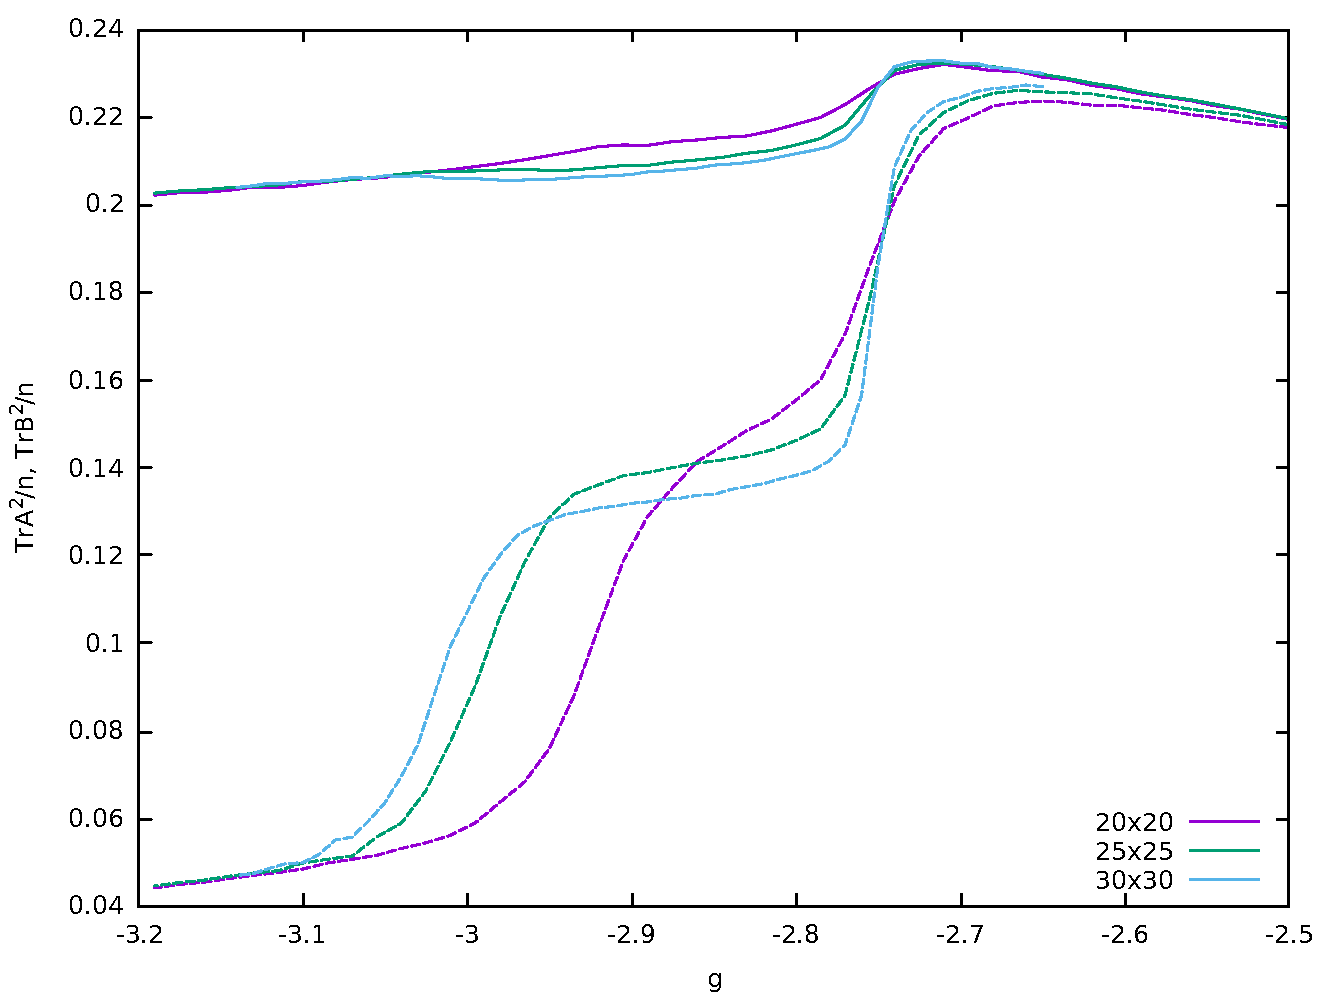
\includegraphics[width=1\linewidth]{fig/ab.pdf}
\caption{$\Tr A^2/n$ (dotted lines) and $\Tr B^2/n$ (solid lines) versus coupling constant $g$ for $n = 20 \ (\text{purple}), 25 \ (\text{green}), 30 \ (\text{blue})$ at the phase transition.}
\label{fig:ab}
\end{figure}
\newpage

%\section{Future directions}\label{future}
%\input{spvar_bare}
%\input{matter_bare}
%\input{RHMC_bare}

\section*{Appendix A: Notation}
\begin{enumerate}
\item To avoid dealing with both Hermitian and anti-Hermitian matrices in Eq.(\ref{eq:dirac_bad}), it is convenient to redefine $i \tilde{L}_j \equiv L_j$ and $\tilde{\alpha}_j \equiv i \alpha_j$. Eq.(\ref{eq:dirac_bad}) becomes:
\begin{equation}
D = \sum_j \tilde{\alpha}_j \otimes [\tilde{L}_j, \cdot ] + \sum_k \tau_k \otimes \{H_k, \cdot \}
\end{equation}
and all the matrices are Hermitian.
\item Commutators and anti-commutators are represented in matrix form as:
$$[A, \cdot ] = A \otimes I - I \otimes A^T$$
$$\{A, \cdot \} = A \otimes I + I \otimes A^T.$$
As a shorthand, the following notation will be used:
\begin{equation}\label{eq:acomm}
[A, \cdot ]_{\epsilon} \equiv A \otimes I + \epsilon \ I \otimes A^T.
\end{equation}
\end{enumerate}
The final form of Eq.(\ref{eq:dirac_bad}) is then:
\begin{equation}\label{eq:dirac}
D = \sum_{i \in I} \omega_i \otimes [ M_i, \cdot ]_{\epsilon_i}
\end{equation}
for Hermitian matrices $M_i$, with $\omega_i \in \{ \tilde{\alpha}_j \} \cup \{ \tau_k \}$, and $\epsilon_i = \pm 1$ depending on $\omega_i$ being a $\tau$ matrix or a $\tilde{\alpha}$ matrix.

\section*{Appendix B: Matrix derivatives} \label{sec:matder}
Let $A \in M_n(\mathbb{C})$ and $f(A)$ be a complex valued function of $A$. The derivative of $f$ with respect to $A$ is defined in components as the $n \times n$ matrix:
\begin{equation}
\left(\frac{\partial f}{\partial A}\right)_{lm} \equiv \frac{\partial f}{\partial A_{lm}}.
\end{equation}
The two special cases of interest here are:
\begin{equation}
\frac{\partial \Tr A}{\partial A} = I
\end{equation}
\begin{equation}
\frac{\partial \Tr AB}{\partial A} = B^T.
\end{equation}

\section*{Appendix C}
The explicit form of $\mathcal{B}_k(i,i,k), \ \mathcal{B}_k(i,k,i)$ and $\mathcal{B}_k(k,k,k)$ is given.
\begin{align}
\mathcal{B}_k(i,i,k) &= \Tr(\omega_k \omega_i \omega_i \omega_k)A(k, i, i, k)^T = CA(k,i,i,k)^T \notag \\ 
\mathcal{B}_k(i,k,i) &= \Tr(\omega_k \omega_i \omega_k \omega_i)A(k, i, k, i)^T \notag \\
\mathcal{B}_k(k,k,k) &= \Tr(\omega_k \omega_k \omega_k \omega_k)A(k, k, k, k)^T = CA(k,k,k,k)^T \notag
\end{align}
where $C$ is the dimension of the Clifford module and the $A$ matrices are:
\begin{align}
A(k,i,i,k) = \ &n [1+\dagger] M_i^2 M_k + \notag \\
&2\epsilon_k I \Tr M_i^2 M_k + \notag \\
&2\epsilon_i \Tr M_i [1 + \dagger] M_i M_k + \notag \\
&4\epsilon_k \epsilon_i M_i \Tr M_i M_k + \notag \\
&2\epsilon_k M_i^2 \Tr M_k + \notag \\
&2M_k \Tr M_i^2
\end{align}
\begin{align}
A(k,i,k,i) = \ &2n M_i M_k M_i + \notag \\
&2\epsilon_k I \Tr M_i^2 M_k + \notag \\
&2\epsilon_i \Tr M_i [1+\dagger] M_i M_k + \notag \\
&4\epsilon_k \epsilon_i M_i \Tr M_i M_k + \notag \\
&2\epsilon_k M_i^2 \Tr M_k + \notag \\
&2M_k \Tr M_i^2
\end{align}
\begin{align}
A(k,k,k,k) = \ &2n M_k^3 + 2\epsilon_k I \Tr M_k^3 + \notag \\
&6 M_k \Tr M_k^2 + 6\epsilon_k M_k^2 \Tr M_k.
\end{align}

\section*{Appendix D}
Suppose $D$ is a $n \times n$ matrix in which $m$ entries are linearly independent. An arbitrary entry can then be written as:
\begin{equation}
D_{ab} = \sum_{ij} c^{ij}_{ab} D_{ij}
\end{equation}
where $c^{ij}_{ab}$ are coefficients and the sum runs over the independent components. This is the case for fuzzy Dirac operators.\newline
The following identity will be proven:
\begin{equation}
\sum_{ij} D_{ij} \frac{\partial}{\partial D_{ij}} \Tr D^p = p \Tr D^p.
\end{equation}
An explicit calculation gives:
\begin{align}
&\sum_{ij} D_{ij} \frac{\partial}{\partial D_{ij}} \Tr D^p = \sum_{ij} D_{ij} \frac{\partial}{\partial D_{ij}} \sum_{a_1 \cdots a_p} D_{a_1 a_2} \cdots D_{a_p a_1} = \notag \\ 
&= \sum_{ij} D_{ij} \sum_{a_1 \cdots a_p} \left( c^{ij}_{a_1 a_2} D_{a_2 a_3} \cdots D_{a_p a_1} + \cdots + D_{a_1 a_2} \cdots D_{a_{p-1} a_p} c^{ij}_{a_p a_1} \right) = \notag \\
&= \sum_{a_1 \cdots a_p} \left( \left(\sum_{ij} c^{ij}_{a_1 a_2} D_{ij}\right) D_{a_2 a_3} \cdots D_{a_p a_1} + \cdots + D_{a_1 a_2} \cdots D_{a_{p-1} a_p} \left( \sum_{ij} c^{ij}_{a_p a_1} D_{ij} \right) \right) = \notag \\
&= p \sum_{a_1 \cdots a_p} D_{a_1 a_2} \cdots D_{a_p a_1} = p \Tr D^p 
\end{align}

\begin{thebibliography}{99} % alternatively use BibTeX

\bibitem{barrettLOR}
J.~W. Barrett,
``Lorentzian version of the noncommutative geometry of the standard model of particle physics'',
{\it J. Math.\ Phys.\ \bf 48}, 012303 (2007).

\bibitem{barrett}
J.~W. Barrett,
``Matrix geometries and fuzzy spaces as finite spectral triples'',
{\it J. Math.\ Phys.\ \bf 56}, 082301 (2015).

\bibitem{barrettglaser}
J.~W. Barrett and L. Glaser,
``Monte Carlo simulations of random non-commutative geometries'',
{\it J. Phys.\ A\ \bf 49}, 24, 245001 (2016).

\bibitem{betan}
M. Betancourt,
``A Conceptual Introduction to Hamiltonian Monte Carlo'',
(arXiv:1701.02434v1, 2017).

\bibitem{bhat}
U. Bhat, M. Shrestha and L. H\'ebert-Dufresne,
``Exotic phase transitions of k-cores in clustered networks'',
{\it Phys.\ Rev. \ E \ \bf 95}, 012314 (2017).

\bibitem{bittner}
E. Bittner and W. Janke,
``Parallel-tempering cluster algorithm for computer simulations of critical phenomena'',
{\it Phys.\ Rev. \ E \ \bf 84}, 036701 (2011).

\bibitem{connesSAP}
A.~H. Chamseddine and A. Connes,
``The spectral action principle'',
{\it Commun.\ Math.\ Phys. \ \bf 186}, 731--750 (1997).

\bibitem{connesNEUT}
A.~H. Chamseddine, A. Connes and M. Marcolli,
``Gravity and the standard model with neutrino mixing'',
{\it Adv.\ Theor. \ Math.\ Phys. \ \bf 11}, 991--1089 (2007).

\bibitem{pol}
P.  Colomer-de-Sim\'on and M. Bogu\~n\'a,
``Double Percolation Phase Transition in Clustered Complex Networks'',
{\it Phys.\ Rev. \ X \ \bf 4}, 041020 (2014).

\bibitem{connesGRAVMAT}
A.~Connes,
``Gravity coupled with matter and the foundation of noncommutative geometry'',
{\it Commun.\ Math.\ Phys. \ \bf 183}, 1, 155--176 (1996).

\bibitem{connesRECON}
A.~Connes,
``On the spectral characterization of manifolds'',
{\it J. Noncommut.\ Geom. \ \bf 7}, 1--82 (2013).

\bibitem{masterthesis}
M. D'Arcangelo,
{\it Random Non-Commutative Geometries\/}
(Unpublished master's thesis, 2017).

\bibitem{duane}
S. Duane, A.~D. Kennedy, B.~J. Pendleton and D. Roweth,
``Hybrid Monte Carlo'',
{\it Phys.\ Lett. \ B \ \bf 195}, 216--222 (1987).

\bibitem{earl}
D.~J. Earl and M.~W. Deem,
``Parallel tempering: Theory, applications, and new perspectives'',
{\it Phys.\ Chem. \ Chem. \ Phys. \bf 7}, 3910--3916 (2005).

\bibitem{erdos}
P. Erd\H os and A. R\'enyi,
``On the Evolution of Random Graphs'',
{\it Publication of the Mathematical Institute of the Hungarian Academy of Sciences\/}
17--61 (1960).

\bibitem{glaser}
L. Glaser,
``Scaling behaviour in random non-commutative geometries'',
{\it J. Phys.\ A\ \bf 50}, 27, 275201 (2017).

\bibitem{hastings}
W.~K. Hastings,
``Monte  Carlo sampling  methods using  Markov chains  and their applications'',
{\it Biometrika\ \bf 57}, 1, 97--109 (1970).

\bibitem{montvay}
I.~Montvay and G. Munster,
{\it Quantum Fields on a Lattice\/}
(Cambridge University Press, 2009).

\bibitem{neal}
R.~M. Neal,
{\it Handbook of Markov Chain Monte Carlo\/}
(Chapman \& Hall / CRC Press, 2011).

\bibitem{suijlekom}
W.~D. Suijlekom,
{\it Noncommutative Geometry and Particle Physics\/}
(Springer, 2014).

\bibitem{swendsen}
R.~H. Swendsen and J.~-S. Wang,
``Replica Monte Carlo Simulation of Spin-Glasses'',
{\it Phys.\ Rev. \ Lett. \ \bf 57}, 1, 2607 (1986).

\bibitem{zukovic}
M. \v Zukovi\v c and G. Kalagov,
``Magnetic quasi-long-range ordering in nematic systems due to competition between higher-order couplings'',
{\it Phys.\ Rev. \ E \ \bf 97}, 052101 (2018).


\end{thebibliography}

\end{document}
